\documentclass{TIJMUjiaoanSY}
\pagestyle{empty}


\begin{document}


%课程名称
\kecheng{系统生物学}
%实验名称
\shiyan{实验一\ 测序数据的质量控制与预处理}
%教师姓名
\jiaoshi{伊现富}
%职称
\zhicheng{讲师}
%教学日期(格式:XXXX年XX月XX日XX时-XX时)
\riqi{2017年3月8日13:30-16:30}
%授课对象(格式:XXX系XXXX年级XX班(硕/本/专科))
\duixiang{生物医学工程与技术学院2014级生信班(本)}
%实验人数
\renshu{30}
%实验类型
\leixing{验证型}
%实验分组
\fenzu{一人一机}
%学时数
\xueshi{3}
%教材版本
\jiaocai{系统生物学实验讲义(自编教材)}


%教案首页
\firstHeader
\maketitle
\thispagestyle{empty}

\mudi{
\begin{itemize}
  \item 掌握二代测序数据的FASTQ格式。
  \item 熟悉FastQC和FASTX-Toolkit等工具的使用方法。
  \item 熟悉Galaxy的使用方法。
  \item 了解FastQC输出结果的含义。
\end{itemize}
}

\fenpei{
\begin{itemize}
  \item (10')FASTQ格式:回顾存储二代测序数据的FASTQ格式。
  \item (10')质控与预处理:回顾二代测序数据分析流程中质控与预处理。
  \item (10')FastQC和FASTX-Toolkit:回顾FASTQC和FASTX-Toolkit的基本用途。
  \item (120')实验操作:对以FASTQ格式存储的二代测序数据进行质量控制与预处理。
\end{itemize}
}

\cailiao{
\begin{itemize}
  \item 实验材料:以FASTQ格式存储的二代测序数据。
  \item 主要仪器:联网的计算机。
  \item 分析工具:Galaxy,FastQC,TASTX-Toolkit。
\end{itemize}
}

\zhongdian{
\begin{itemize}
  \item 难点:FASTQ格式;解决策略:通过实例进行讲解。
  \item 重点:FastQC和FASTX-Tollkit的使用;解决策略:根据资料进行学习,通过练习熟练掌握。
\end{itemize}
}

\sikao{
\begin{itemize}
  \item 解释存储二代测序数据的FASTQ格式。
  \item 列举二代测序数据质控和预处理的主要内容。
  \item 如何对二代测序数据进行质控和预处理?
\end{itemize}
}

\cankao{
\begin{itemize}
  \item FastQC
  \item FASTX-Toolkit
  \item Galaxy
\end{itemize}
}

\firstTail


%教案续页
\newpage
\otherHeader

\noindent
\begin{enumerate}
  \item FASTQ格式(10分钟)
    \begin{figure}[ht]
      \centering
      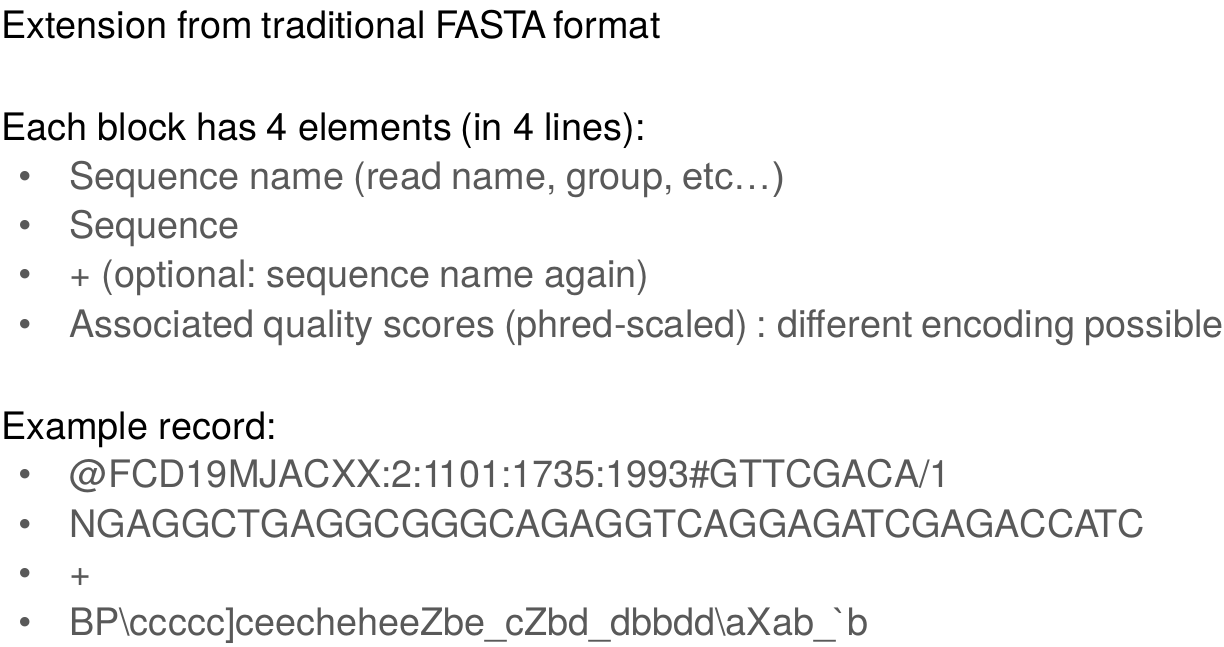
\includegraphics[width=0.45\textwidth]{c2_format_fastq_06.png}
      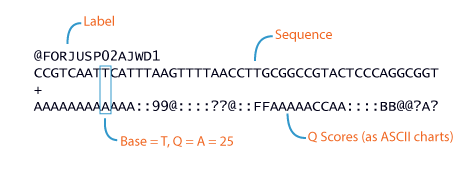
\includegraphics[width=0.5\textwidth]{c2_format_fastq_11.png}
    \end{figure}

  \item 质控与预处理(10分钟)
\parpic[fr]{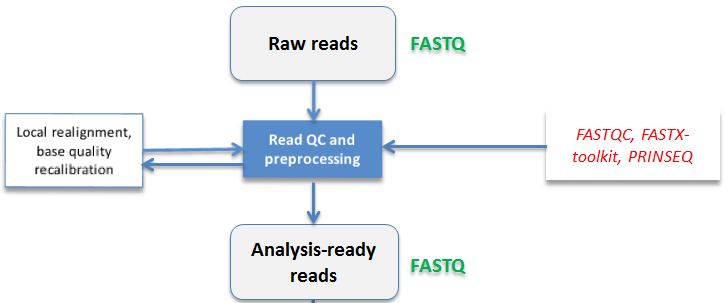
\includegraphics[width=8.5cm]{c2_workflow_ngs_031.png}}
    \begin{enumerate}
      \item 质量控制
        \begin{itemize}
          \item Identify poor/bad sample
          \item Identify contaminates
        \end{itemize}
      \item 预处理
        \begin{itemize}
          \item Trimming: remove bad bases from read
          \item Filtering: remove bad reads from library
        \end{itemize}
    \end{enumerate}

  \item FastQC和FASTX-Toolkit(10分钟)
    \begin{multicols}{2}
      \begin{enumerate}
        \item FastQC: quality control tool
          \begin{itemize}
            \item Basic statistics
            \item Per base sequence quality
            \item Per tile sequence quality
            \item Per sequence quality content
            \item Per base sequence content
            \item ...
         \end{itemize}
       \item FASTX-Toolkit: FASTA/FASTQ preprocessing
         \begin{itemize}
           \item Remove linker/adapter sequences
           \item Trim low quality reads at the end of the read
           \item Filter sequences based on quality
           \item ...
         \end{itemize}
      \end{enumerate}
    \end{multicols}

  \item 实验操作(120分钟)
    \begin{enumerate}
      \item Upload data to Galaxy\textcolor{red}{(比较导入数据的不同方法;注意参数的设定)}
      \item Checking read quality with FastQC\textcolor{red}{(理解输出结果中每一部分的含义)}
      \item Convert FASTQ quality to sanger\textcolor{red}{(为什么要进行质量编码的转换)}
      \item Preprocessing with FASTX-Toolkit\textcolor{red}{(结合FastQC的结果进行预处理)}
      \item Clean adapter containing reads from FASTQ data\textcolor{red}{(结合FastQC的结果进行预处理)}
      \item 探索``NGS: QC and manipulation"中的其他工具\textcolor{red}{(同一个任务可以选用不同的工具)}
    \end{enumerate}
\end{enumerate}


\otherTail


\end{document}

